\section{Message Passing}

\definecolor{darkgreen}{rgb}{0,0.6,0}

\mode<presentation>{
\begin{frame} 
    \begin{center} \huge
        \secname
    \end{center}
    \begin{center}
    a compact look-up-table
    \end{center}
    
    \begin{center}
		
\includegraphics[width=0.3\textwidth]{img/meme_msg}
    \end{center}
\end{frame}
}

\subsection{Overview}

\begin{frame}\frametitle{Message Passing: Overview}

\begin{itemize}
\item essentially storage of local computations for faster look-up
\item will be used to calculate conditional probabilities in a junction tree by only using local ``simpler'' computations.
\item scales well with no. of variables.
\end{itemize}

\end{frame}

\subsection{Procedure}

% -----------------------------------------------------------------------------
\begin{frame} \frametitle{\secname: \subsecname}
	%\iitem{a third pass can calculate all other marginals}
	\begin{minipage}[c]{12.1cm}
		\begin{minipage}[][1cm][c]{8cm}
			\begin{itemize}
				\item first pass from root to leaves: \textcolor{red}{``request''}\\
				selecting the root (for tree structures any node can be the root, so not sensitive to choice of root node)
			\end{itemize}
		\end{minipage}
		\hfill \raisebox{-4mm}{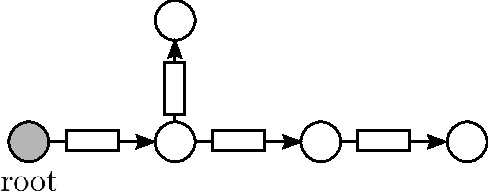
\includegraphics[width=4cm]{img/section3_fig20}} \\
		\begin{minipage}[c]{8cm}
			\begin{itemize}
				\item second pass from leaves to root: \textcolor{blue}{``collect''}\\
				collect messages from other neighbors
			\end{itemize}
		\end{minipage}
		\hfill \raisebox{-8mm}{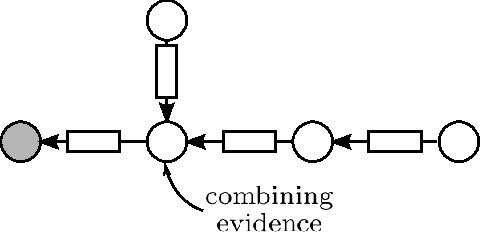
\includegraphics[width=4cm]{img/section3_fig21}} \\
		\pause
		\begin{minipage}{8cm}
			\begin{itemize}
				\item a third pass can calculate all other \\
					marginals: \textcolor{darkgreen}{``distribute''}\\
					third pass from root to leaves to compute the remaining messages.
			\end{itemize}
		\end{minipage}
		\hfill \raisebox{-6mm}{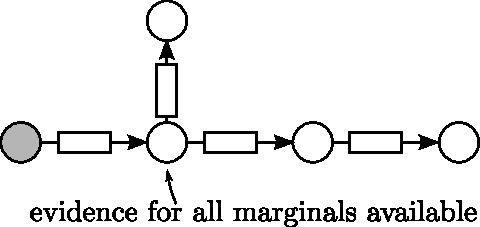
\includegraphics[width=4cm]{img/section3_fig22}} \\
	\end{minipage}
\end{frame}

\subsection{The sum-product algorithm}
% -----------------------------------------------------------------------------
\begin{frame} \frametitle{\subsecname}
	\vspace{-4mm}
	%\begin{minipage}{12cm}
		%\begin{minipage}{6.5cm}
			%\vspace{5mm}
			%\includegraphics[height=3.5cm]{img/tree_inference_product_message_v2}
			%\begin{itemize}
				%\item product message from $X_m$ to $f_s$
			%\end{itemize}
		%\end{minipage}
		%\hfill
		%\visible<2>{\begin{minipage}{6cm}
			%\hfill
			%\includegraphics[height=3.65cm]{img/tree_inference_sum_message_v2}
			%\vspace{2mm} 
			%\begin{itemize}
				%\item sum message from $f_s$ to $X_i$
			%\end{itemize}
		%\end{minipage}}
	%\end{minipage}
    
    Defining the messages between the different types of nodes in a bipartite graph (e.g. separators and cliques)\footnote{for details, see Ch. 8.4.4, p. 402 in \citep{bishop2006pattern}}

	%\hspace{-4mm}
	\begin{align}
		\mu_{X_m \to f_s}(X_m) &\;:=&&\kern-4ex
			\kern-3ex\prod_{l \in \text{neighbor}(X_m) \setminus\{f_s\}}\kern-3ex
			\mu_{f_l \to X_m}(X_m) \tag{product}\\[1mm] 
		\visible<3>{
		\mu_{f_s \to X_i}(X_i) &\;:=&&\kern-3ex 
			\sum_{x_m, \ldots, x_M}\kern-2ex f_s(X_i, x_m,\ldots, x_M) 
			\kern-5ex\prod_{k \in \text{neighbor}(f_s)\setminus\{X_i\}}\kern-5ex 
			\mu_{X_k \to f_s}(x_k) 
			\only<1,2>{\nonumber\hspace{10mm}}
			\only<3>{\tag{sum}}
		}
        \label{eq:sumproduct}
	\end{align}
	
	\mode<presentation>{
	\only<2>{
	\svspace{-15mm}
	\begin{center}
		
\includegraphics[width=0.3\textwidth]{img/meme_product}
	\end{center}
	}
	}
	
	\mode<article>{
	\begin{itemize}
	\item The arguments of the messages follow the variables in the separator node.
	\item For the \emph{product} formula, the product runs over all clique potentials that are neighbors of the separator $X_m$, \underline{except} for $f_s$ that the message is going to.
	\item For the \emph{sum} formula, the sum takes care of marginalizing over all the variables that are present in the outgoing clique potential $f_s$ but are absent from the variables of the target separator $X_i$. This is weighted by the product of messages that arrive at $f_s$ from \underline{other} neighbors (i.e. we exclude the separator that the message is going to).
	\end{itemize}
	}
\end{frame}
